%**************************************************************************
%* SpringSim 2019 Author Kit
%*
%* Word Processing System: TeXnicCenter and MiKTeX
%*
%**************************************************************************
\documentclass{scspaperproc}

\usepackage{latexsym}
\usepackage{graphicx}
\usepackage{mathptmx}

%
%****************************************************************************
% AUTHOR: You may want to use some of these packages. (Optional)
%\usepackage{amsmath}
%\usepackage{amsfonts}
%\usepackage{amssymb}
%\usepackage{amsbsy}
%\usepackage{amsthm}
%****************************************************************************


%
%****************************************************************************
% AUTHOR: If you do not wish to use hyperlinks, then just comment
% out the hyperref usepackage commands below.

%% This version of the command is used if you use pdflatex. In this case you
%% cannot use ps or eps files for graphics, but pdf, jpeg, png etc are fine.

\usepackage[pdftex,colorlinks=true,urlcolor=blue,citecolor=black,anchorcolor=black,linkcolor=black]{hyperref}

%% The next versions of the hyperref command are used if you adopt the
%% outdated latex-dvips-ps2pdf route in generating your pdf file. In
%% this case you can use ps or eps files for graphics, but not pdf, jpeg, png etc.
%% However, the final pdf file should embed all fonts required which means that you have to use file
%% formats which can embed fonts. Please note that the final PDF file will not be generated on your computer!
%% If you are using WinEdt or PCTeX, then use the following. If you are using
%% Y&Y TeX then replace "dvips" with "dvipsone"

%% \usepackage[dvips,colorlinks=true,urlcolor=blue,citecolor=black,%
%% anchorcolor=black,linkcolor=black]{hyperref}

%% The use of the long citation format (e.g. "Brown and Edwards (1993)" rather than "[5]") and at the same
%% time using the hyperref package can lead to hard to trace bugs in case the citation is broken accross the
%% line (usually this will mark the entire paragraph as a hyperlink (clickable) which is easily noticeable and fixed
%% if using colorlinks, but not if the color is black -- as it is now). Worse yet, if a citation spans page boundary,
%% LaTeX compilation can fail, with an obscure error message. Since this depends a lot on the flow of the text
%% and wording, these bugs come and go and can be extremely hard for a beginner to trace. The error
%% message can look like this:
%%
%%    ! pdfTeX error (ext4): \pdfendlink ended up in different nesting level than \pdfstartlink.
%%    \AtBegShi@Output ...ipout \box \AtBeginShipoutBox 
%%    \fi \fi 
%%    l.174 
%%    ! ==> Fatal error occurred, no output PDF file produced!
%%
%% and can be universally fixed by putting an \mbox{} around the citation in question (in this case, at line 174)
%% and maybe adapting the wording a little bit to improve the paragraph typesetting, which is perhaps not
%% immediately obvious.
%****************************************************************************

%
%****************************************************************************
%*
%* AUTHOR: YOUR CALL!  Document-specific macros can come here.
%*
%****************************************************************************

\usepackage{float}
\usepackage{subcaption}
\usepackage{minted}
\usepackage{verbatim}

%#########################################################
%*
%*  The Document.
%*
\begin{document}

%***************************************************************************
% AUTHOR: AUTHOR NAMES GO HERE
% FORMAT AUTHORS NAMES Like: Author1, Author2 and Author3 (last names)
%
%		You need to change the author listing below!
%               Please list ALL authors using last name only, separate by a comma except
%               for the last author, separate with "and"
%
\SCSpagesetup{Thaler, Siebers and Altenkirch}

% AUTHOR: Uncomment ONE of these correct conference names.
%\def\SCSconferenceacro{SpringSim}
\def\SCSconferenceacro{SummerSim}
%\def\SCSconferenceacro{AutumnSim}
%\def\SCSconferenceacro{PowerPlantSim}

% AUTHOR: Set the correct year of the conference.
\def\SCSpublicationyear{2019}

% AUTHOR: Set the correct month and dates; the dates are separated by a single minus sign
% with no spaces and no leading zeros, the month is a full name (e.g. April) with the first letter
% capitalized. For example, "April 8-13".
\def\SCSconferencedates{July 22-July 24}

% AUTHOR: Set the correct venue in the form "City, State, Country", for example "Los Angeles, CA, USA".
\def\SCSconferencevenue{Berlin, Germany}

% AUTHOR: Uncomment ONE of the track/symposium names where you are going to submit. Please, do NOT change.
% In case your symposium is not on this list, please DO contact your symposium chair.
\def\SCSsymposiumacro{ANSS} % Annual Simulation Symposium
%\def\SCSsymposiumacro{CNS} % Communications and Networking Simulation Symposium
%\def\SCSsymposiumacro{HPC} % High Performance Computing Symposium
%\def\SCSsymposiumacro{TMS/DEVS} % Symposium on Theory of Modeling and Simulation
%\def\SCSsymposiumacro{ADS} % Agent-Directed Simulation
%\def\SCSsymposiumacro{MSCIAAS} % Modeling and Simulation of Complexity in Intelligent, Adaptive and Autonomous Systems
%\def\SCSsymposiumacro{MSM} % Modeling and Simulation in Medicine
%\def\SCSsymposiumacro{Mod4Sim} % Model-driven Approaches for Simulation Engineering Symposium
%\def\SCSsymposiumacro{Tutorial} % Tutorial Track
%\def\SCSsymposiumacro{WIP} % WIP Track
%\def\SCSsymposiumacro{Poster/Colloquium} % Poster Session and Student Colloquium
%\def\SCSsymposiumacro{MobileApp} % Student M\&S Mobile App Competition
%\def\SCSsymposiumacro{SPECTS} % Symposium on Performance Evaluation of Computer and Telecommunication Systems
%\def\SCSsymposiumacro{SCSC} % Summer Computer Simulation Conference
%\def\SCSsymposiumacro{ICBGM} % International Conference on Bond-Graph Modeling
%\def\SCSsymposiumacro{Fossil} % Fossil Power Track
%\def\SCSsymposiumacro{Nuclear} % Nuclear Agent Power Track

% AUTHOR: Enter the title, all letters in upper case

\newminted[HaskellCode]{haskell}{fontsize=\footnotesize}

% Title portion. Note the short title for running heads
\title{The Agents New Cloths \\ \small{Towards Pure Functional Programming in ABS}}
%\subtitle{Towards Pure Functional Programming in ABS}

% AUTHOR: Enter the authors of the article, see end of the example document for further examples
\author{
\\%To level with the author block on the right.
Jonathan Thaler \\ 
Peer Olaf Siebers \\ [12pt] 
School Of Computer Science \\
University of Nottingham \\
7301 Wollaton Rd \\
Nottingham, United Kingdom \\
\{jonathan.thaler,peer-olaf.siebers\}@nottingham.ac.uk\\
}

\maketitle

\section*{Abstract}
%NOTE we target Summer Simulation Conference: http://scs.org/summersim/ with the sub-track on Agent-based Modeling and Simulation (ABMS) 

TODO

\textbf{Keywords:} Agent-Based Simulation, Functional Programming, Haskell, Concurrency, Parallelism, Property-Based Testing, Validation \& Verification.

\maketitle

\section{Introduction}
There exists a large number of simulation packages which allow the convenient creation of System Dynamics simulations by straight-forward visual diagram creation. One simply creates stocks and flows, connects them, specifies the flow-rates and initial parameters and then runs the model. An example for such a visual diagram creation in the simulation package AnyLogic can be seen in Figure \ref{fig:sir_stockflow_diagram}.

\begin{figure}
	\centering
	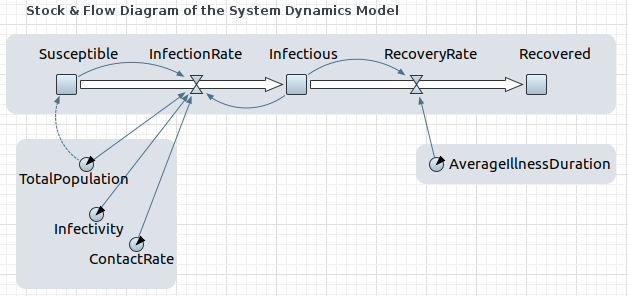
\includegraphics[width=.5\textwidth, angle=0]{./fig/SIR_SD_STOCKFLOW_DIAGRAMM.png}
	\caption{Visual System Dynamics Diagram of the SIR model in AnyLogic Personal Learning Edition 8.3.1.}
	\label{fig:sir_stockflow_diagram}
\end{figure}

Still, implementing System Dynamics directly in code is not as straight forward and involves numerical integration which can be quite tricky to get right. Thus, the aim of this paper is to look into how System Dynamics models can be implemented in code correctly without the use of a simulation package. We use the well known SIR model \cite{kermack_contribution_1927} from epidemiology to demonstrate our approach.

Our language of choice is Haskell because it emphasises a declarative programming style in which one describes \textit{what} instead of \textit{how} to compute. Further it allows to rule out interference with non-deterministic influences or side-effects already at compile-time. This is of fundamental importance for System Dynamics because it behaves completely deterministic and involves no stochastics or non-determinism whatsoever. Also, we make use of Functional Reactive Programming which allows to express continuous-time systems in a functional way. 

We show that by this approach we can arrive at correct-by-construction implementations of System Dynamic models. This means that the correctness of the code is obvious because we have closed the gap between the model specification and its implementation. Thus, the contribution of the paper is the demonstration of how to implement correct-by-construction System Dynamics simulations using Haskell and Functional Reactive Programming.

\section{Case-Study: Pure Functional SugarScape}
TODO

why sugarscape
- original sugarscape sparked ABS and use of OOP, therefore 
- quite complex model, will challenge implementation techniques

\footnote{The code is freely accessible from \url{https://github.com/thalerjonathan/phd/tree/master/public/towards/code}}

\cite{weaver_replicating_nodate}

page 28, footnote 16: we can guarantee that in haskell at compile time

\section{Replication Issues}
\subsection{Terracing}
Our implementation reproduce the terracing phenomenon as described on page TODO in Animation and as can be seen in the NetLogo implementation as well. We implemented a property-test in which we measure the closeness of agents to the ridge: counting the number of same-level sugarscells around them and if there is at least one lower then they are at the edge. If a certain percentage is at the edge then we accept terracing. The question is just how much, this we estimated from tests and resulted in 45\%. Also, in the terracing animation the agents actually never move which is because sugar immediately grows back thus there is no need for an agent to actually move after it has moved to the nearest largest cite in can see. Therefore we test that the coordinates of the agents after 50 steps are the same for the remaining steps.

\subsection{Carrying Capacity}
Our simulation reached a steady state (variance < 4 after 100 steps) with a mean around ~182. Epstein reported a carrying capacity of 224 (page 30) and the NetLogo implementations carrying capacity fluctuates around 205 which both were thus significantly higher than ours. Something was definitely wrong - the carrying capacity has to be around 200 (we trust in this case the NetLogo implementation and deem 224 an outlier).

After inspection of the netlogo model we realised that we implicitly assumed that the metabolism range is \textit{continuously} uniformly randomized between 1 and 4 but this seemed not what the original authors intended: in the netlogo model there were a few agents surviving on sugarlevel 1 which was never the case in ours as the probability of drawing a metabolism of exactly 1 is 0 when drawing from a continuous range. We thus changed our implementation to draw discrete. Note that this actually makes sense as massive floating-point number calculations were quite expensive in the mid 90s (e.g. computer games ran still on CPU only and exploited various  clever tricks to avoid the need of floating point calculations whenever possible) when SugarScape was implemented which might have been a reason for the authors to assume it implicitly.

This partly solved the problem, the carrying capacity was now around 204 which is much better than 182 but still a far cry from 210 or even 224. After adjusting the order in which agents apply the sugarscape rules, (by looking at the code of the netlogo implementation), we arrived at a comparable carrying capacity of the netlogo implementation: agents first make their move and harvest sugar and only after this the agents metabolism is applied (and ageing in subsequent experiments).

For regression-tests we implemented a property-test which tests that the carrying capacity of 100 simulation runs lies within a 95\% confidence interval of a 210 mean. TODO: variance test. These values are quite reasonable to assume, when looking at NetLogo - again we deem the reported Carrying Capacity of 224 in the Book to be an outlier / part of other details we don't know.

TODO: do a replication experiment with NetLogo (is it possible?)

\subsection{Wealth Distribution}
By visual comparison we validated that the wealth distribution (page 32-37) becomes strongly skewed with a Histogram showing a fat tail, power-law distribution where very few agents are very rich and most of the agents are quite poor. We compute the skewness and kurtosis of the distribution which is around a skewness of 1.5, clearly indicating a right skewed distribution and a kurtosis which is around 2.0 which clearly indicates the lst histogram of Animation II-3 on page 34. Also we compute the gini-coefficient and it varies between 0.47 and 0.5 - this is accordance with Animation II-4 on page 38 which shows a gini-coefficient which stabilises around 0.5 after. 
We implemented a regression-test testing skewness, kurtosis and gini-coefficients of 100 runs to be within a 95\% confidence interval of a two-sided t-test using an expected skewness of 1.5, kurtosis of 2.0 and gini-coefficient of 0.48.

\subsection{Migration}
With the information provided by \cite{weaver_replicating_nodate} we could replicate the waves as visible in the NetLogo implementation as well. Also we propose that a vision of 10 is not enough yet and shall be increased to 15 which makes the waves very prominent and keeps them up for much longer - agent waves are travelling back and forth between both sugarscape peaks. We haven't implemented a regression-test for this property as we couldn't come up with a reasonable straight forward approach to implement it.

\subsection{Polution and Diffusion}
With the information provided by \cite{weaver_replicating_nodate} we could replicate the polution behaviour as visible in the NetLogo implementation as well. We haven't implemented a regression-test for this property as we couldn't come up with a reasonable straight forward approach to implement it.

Note that we spent quite a lot of time of getting this and the terracing properties right because they form the very basics of the other ones which follow so we had to be sure that those were correct otherwise validating would have been much more difficult.

\subsection{Order of Rules}
order in which rules are applied is not specified and might have an impact on dynamics e.g. when does the agent mate with others: is it after it has harvested but before metabolism kicks in?

\section*{Acknowledgments}
The authors would like to thank

% Please don't change the bibliographystyle style
\bibliographystyle{scsproc}
% AUTHOR: Include your bib file here
\bibliography{../../../references/phdReferences.bib}

% what a waste of space
%\section*{Author Biographies}
%\textbf{\uppercase{JONATHAN THALER}} is a PhD. student.
%\textbf{\uppercase{PEER-OLAF SIEBERS}} is Jonathans Supervisor.

\end{document}